\documentclass[12pt,journal,onecolumn]{IEEEtran}
%\documentclass[conference]{IEEEtran} \documentclass[12pt,a4paper]{article}
%
\usepackage[T1]{fontenc}
\usepackage{graphicx}
\addtolength{\topmargin}{0.02in}
\addtolength{\textheight}{-0.02in}
\setlength{\marginparwidth}{2cm}
\usepackage[ disable,     % hide all todos
    % obeyDraft,   % show todos only in draft mode obeyFinal,   % hide todos if
    % in final mode textsize=footnotesize,
    textwidth=.9\marginparwidth, colorinlistoftodos, prependcaption,
    linecolor=green,backgroundcolor=green!25,bordercolor=green ]{todonotes}
\usepackage{amsfonts}
\usepackage{mathtools}
%\usepackage[bookmarks=false, hidelinks, linktocpage=false,
%    breaklinks=false,draft]{hyperref}
\usepackage[bookmarks=false, hidelinks, linktocpage=false,
    breaklinks=true]{hyperref}
\usepackage{xurl}
\usepackage{makecell}
\usepackage{xcolor}
\usepackage{algorithm}
\usepackage{algpseudocodex}
\usepackage{float}
\usepackage{nicefrac}
\usepackage{microtype}
\usepackage{adjustbox}
\usepackage{booktabs}
\usepackage{tabularx}
\usepackage[capitalise]{cleveref}
\usepackage[super]{natbib}


\usepackage{listings}
\usepackage{xcolor}
\usepackage{xurl}

% Define colors for syntax highlighting
\definecolor{codegreen}{rgb}{0,0.6,0}
\definecolor{codegray}{rgb}{0.5,0.5,0.5}
\definecolor{codepurple}{rgb}{0.58,0,0.82}
\definecolor{backcolour}{rgb}{0.95,0.95,0.92}

% Configure listings style
\lstdefinestyle{mystyle}{
    backgroundcolor=\color{backcolour},
    commentstyle=\color{codegreen},
    keywordstyle=\color{magenta},
    numberstyle=\tiny\color{codegray},
    stringstyle=\color{codepurple},
    basicstyle=\ttfamily\footnotesize,
    breakatwhitespace=false,
    breaklines=true,
    captionpos=b,
    keepspaces=true,
    numbers=left,
    numbersep=5pt,
    showspaces=false,
    showstringspaces=false,
    showtabs=false,
    tabsize=2
}
\lstset{style=mystyle}



\makeatletter
\if@todonotes@disabled \else
% todonotes is enabled, increase paper size to get bigger margins
\paperwidth=\dimexpr \paperwidth + 6cm\relax
\oddsidemargin=\dimexpr\oddsidemargin + 3cm\relax
\evensidemargin=\dimexpr\evensidemargin + 3cm\relax \marginparwidth=\dimexpr
\marginparwidth + 3cm\relax \let\oldtitle\title
\renewcommand{\title}[1]{\oldtitle{#1\(_{\colorbox{red!20}{\tiny disable
todos}}\)}}
\fi
\makeatother

% For ORCID support in IEEE format
\usepackage{orcidlink}

\begin{document}
%
\title{ACMEMobility\\
[0.5ex] \large Progetto di Architetture Software a Microservizi, Università di Bologna,
2025--2026}

% IEEE format doesn't use running titles

\author{
  \small
  \begin{tabular}{c c c}
    \begin{minipage}[t]{0.3\textwidth}\centering \IEEEauthorblockN{Daniele
      D'Ugo}\\
      \IEEEauthorblockA{daniele.dugo@studio.unibo.it \\ Mat.: 0001186581}
    \end{minipage} & 
    \begin{minipage}[t]{0.3\textwidth}\centering \IEEEauthorblockN{Daniele
      D'Ugo}\\
      \IEEEauthorblockA{daniele.dugo@studio.unibo.it \\ Mat.: 0001186581}
    \end{minipage} & 
    \begin{minipage}[t]{0.3\textwidth}\centering \IEEEauthorblockN{Daniele
      D'Ugo}\\
      \IEEEauthorblockA{daniele.dugo@studio.unibo.it \\ Mat.: 0001186581}
    \end{minipage}
  \end{tabular}
}

% IEEE doesn't use \authorrunning

\maketitle              % typeset the header of the contribution
%
%TC:ignore
%\begin{abstract}
%\end{abstract}
%TC:endignore

% IEEE uses different keywords format
%\begin{IEEEkeywords}
%\end{IEEEkeywords}

\section{Introduzione}\label{sec:intro}

Il servizio di noleggio ACMEMobility è stato implementato come un'architettura a
microservizi, tramite \textit{docker compose}, cercando di rispettare tutti i
requisiti del progetto.

\section{Avvio e utilizzo}\label{sec:usage}

L'intera architettura, comprendente tutti i servizi, con il codice nella
cartella \textit{src/}, può essere avviata e gestita tramite i comandi di
\textit{docker compose}; per comodità, sono presenti due script \textit{bash}
(per sistemi Linux). \textit{start.sh} lancia l'infrastruttura:
\begin{lstlisting}[language=Bash]
	# dalla cartella di base del repository
	./src/start.sh
\end{lstlisting}
\textit{down.sh} interrompe i servizi:
\begin{lstlisting}[language=Bash]
	./src/down.sh
\end{lstlisting}


Prima, però, è necessario scaricare la mappa (con dati di OpenStreetMap)
dell'Italia nord-orientale, disponibile al link su geofabrik:
\url{https://download.geofabrik.de/europe/italy/nord-est-latest.osm.pbf}.\\
Il file dovrà essere piazzato in \textit{service-graphhopper/data/}, con nome
del file\\
\mbox{\textit{geofabrik\_italy-nord-est-260517.osm.pbf}}.\\
Da Linux, si può eseguire direttamente, per entrambi i passaggi, il comando:
\begin{lstlisting}[language=Bash]
	# dalla cartella di base del repository
	wget -O service-graphhopper/data/geofabrik_italy-nord-est-260517.osm.pbf \
	https://download.geofabrik.de/europe/italy/nord-est-latest.osm.pbf
\end{lstlisting}


Il flusso delle attività parte sempre dall'utente, che in uno scenario reale
sarebbe un'entità fisica e potrebbe interagire con ACMEMobility tramite
un'applicazione per smartphone. Dunque, abbiamo realizzato uno script in
\textit{python} (\textit{src/user/user.py}) che simula tutte le possibili azioni
che possa compiere, in base agli argomenti utilizzati. Seguono degli esempi per
ogni utilizzo. Usage:
\begin{lstlisting}[language=Bash]
	# dalla cartella di base del repository
	python src/user/user.py
	# Usage: python user.py <action> <user_id> <vehicle_id> [station_id]
	# Actions: scan, reserve, cancel, scan_reserved, park, lock, lock_assistance, steal
\end{lstlisting}

Scansione veicolo (con id \textit{V-01}) per uso immediato, da parte dell'utente
con id \textit{USER-001}:
\begin{lstlisting}[language=Bash]
	python src/user/user.py scan USER-001 V-01
\end{lstlisting}

Prenotazione veicolo per dopo:
\begin{lstlisting}[language=Bash]
	python src/user/user.py reserve USER-001 V-01
\end{lstlisting}

Cancellazione della prenotazione precedente:
\begin{lstlisting}[language=Bash]
	python src/user/user.py cancel USER-001 V-01
\end{lstlisting}

Scansione del veicolo precedentemente prenotato:
\begin{lstlisting}[language=Bash]
	python src/user/user.py scan_reserved USER-001 V-01
\end{lstlisting}

Parcheggio del veicolo (simulazione dell'inserimento del veicolo nel dock della
stazione con id \mbox{\textit{STATION-BOLOGNA-01}}):
\begin{lstlisting}[language=Bash]
	python src/user/user.py park USER-001 V-01 STATION-bologna-01
\end{lstlisting}

Richiesta di fine corsa e, dunque, blocco del veicolo precedentemente
parcheggiato:
\begin{lstlisting}[language=Bash]
	python src/user/user.py lock USER-001 V-01 STATION-bologna-01
\end{lstlisting}

Richiesta di assistenza a fine corsa, in caso di problemi con il blocco:
\begin{lstlisting}[language=Bash]
	python src/user/user.py lock_assistance USER-001 V-01
\end{lstlisting}

Simulazione furto di un veicolo:
\begin{lstlisting}[language=Bash]
	python src/user/user.py steal USER-001 V-01
\end{lstlisting}

Invia un'istruzione a Camunda per eseguire immediatamente il task di timeout
per il tempo di cancellazione di una prenotazione (utile per testare
l'applicazione della penalità):
\begin{lstlisting}[language=Bash]
	python3 src/user/user.py force_timeout USER-001 V-01
\end{lstlisting}


Una volta avviata l'infrastruttura, è possibile accedere alla visualizzazione di
Camunda al link \\
\mbox{\url{http://localhost:8080/camunda/app/cockpit/}}, con username
\textit{demo} e password \textit{demo}.\\
Al link \mbox{\url{http://localhost:4000/map/}}, invece, è possibile
visualizzare una mappa di Bologna, con dei segnali per le stazioni ed eventuali
veicoli in movimento.\\
I veicoli utilizzano coordinate reali e ricevono dei percorsi da un'istanza,
eseguita in locale, di \textit{GraphHopper} --- che espone anche un'interfaccia
web al link \mbox{\url{http://localhost:8989/}}, non particolarmente rilevante
per il progetto.\\
\\
Sono inoltre disponibili altri endpoint, esposti dai vari servizi per
debugging. Seguono quelli più utili per il debugging.\\

Il servizio di ACMEMobility espone il suo database:  
\begin{lstlisting}[language=Bash]
	curl localhost/db
\end{lstlisting}

Ogni stazione espone il suo stato:
\begin{lstlisting}[language=Bash]
	curl localhost:5001/station
	curl localhost:5002/station
	curl localhost:5003/station
	curl localhost:5004/station
	curl localhost:5005/station
\end{lstlisting}


\section{Workflow e artefatti}\label{sec:workflow}

Lo sviluppo del progetto è partito con la modellazione di una coreografia in
BPMN con scopo documentativo. Usandola come schema è stato così possibile
suddividere, tra i membri del gruppo, i compiti di realizzare ulteriori modelli
o i singoli servizi.\\
\\
La coreografia è stata poi gradualmente raffinata, fino a diventare la attuale
coreografia a scopo documentativo (file
\mbox{\textit{docs/diagrams/diagram-collaboration-full.bpmn}}). Essa raffigura
infatti tutti i partecipanti e i loro task, per rendere l'idea di quali feature
debba implementare ogni servizio.\\
Per Camunda è stato modellato un altro diagramma di collaborazione eseguibile\\
(file \mbox{\textit{src/camunda-resources/diagram-collaboration-camunda.bpmn}}),
con la principale differenza che non implementa nel dettaglio tutti i
partecipanti, ma solo il servizio principale di ACMEMobility, che era richiesto
che fosse gestito tramite BPMS.\\
Successivamente, sono stati realizzati un diagramma di documentazione della SOA
in UML, con profilo TinySOA (file \mbox{\textit{docs/diagrams/diagram-SOA.uml}}
e \mbox{\textit{docs/diagrams/diagram-SOA-UML.uml}}), e una coreografia con
sintassi formale, necessaria per le proiezioni della coreografia sui ruoli e per
l'analisi di \textit{connectedness}.\\
\\
I servizi implementati, invece, sono:
\begin{itemize}
	\item ACME (\textit{src/service-acme-worker/}): il worker che implementa i
	service task del BPMS per il core di ACMEMobility, scritto in
	\textit{python} con l'apposito pacchetto per Camunda;
	\item bank (\textit{src/service-bank/}): la banca, in \textit{jolie};
	\item Fleet Management (\textit{src/service-fleet-management/}):
	implementato come un router, in \textit{Nginx}, così che appaia esso stesso
	come un'architettura a microservizi;
	\begin{itemize}
		\item Fleet Management Battery (\textit{src/service-fleet-battery/}):
		microservizio per gestire la batteria dei veicoli, in \textit{python}
		con \textit{Flask};
		\item Fleet Management Tracking (\textit{src/service-fleet-tracking/}):
		microservizio per gestire posizione e informazioni aggiuntive dei
		veicoli, in \textit{python} con \textit{Flask};
	\end{itemize}
	\item grapphopper (\textit{src/service-graphhopper/}): routing service per
	fornire dei percorsi reali ai veicoli, date posizione di partenza e
	destinazione, nonché per visualizzarli in tempo reale; configurato con il
	container \textit{docker} già esistente;
	\item station (\textit{src/service-stations/}): implementazione di una
	singola stazione, in \textit{python} con \textit{Flast};
	\item vehicle (\textit{src/service-vehicle/}): implementazione di un singolo
	veicolo, in \textit{python} con \textit{Flask}.
\end{itemize}

Tutti i servizi sono gestiti tramite un'architettura con
\textit{docker-compose}, che si occupa anche di istanziare molteplici veicoli e
stazioni, con la stessa immagine e implementazione. Il file è scritto come
template in \mbox{\textit{src/docker-compose.template.yml}}; uno script
\textit{bash} (\mbox{\textit{src/bash-scripts/compile-dockercompose.sh}}, già
invocato da \textit{start.sh}) lo lavora, per esempio sostituendo delle
variabili con quelle in \mbox{\textit{src/.env}}, generando quello finale
(\mbox{\textit{src/docker-compose.generated.yml}}). In questo modo, i veicoli e
le stazioni istanziati sono ben riconoscibili poiché generati con identificativi
definiti tramite variabili di ambiente.\\
Per la coreografia in Camunda, come già accennato, tutti i service task sono
implementati tramite un worker in python. Solo delle operazioni banali,
principalmente le condizioni di scelta per i gateway esclusivi, sono
implementate come espressioni \textit{inline}, con sintassi \textit{JUEL}
(\textit{Java Unified Expression Language}), utilizzando delle variabili globali
che vengono configurate dallo stesso worker. L'implementazione esterna, infatti,
fornisce grandi vantaggi nello sviluppo, in termini di gestibilità,
mantenibilità e leggibilità del codice, possibilità di debugging e gestione
coerente e ordinata dei file.\\
Inoltre, tutti i servizi usano \textit{API REST} e comunicano tramite
\textit{http}, ad eccezione della banca, che usa \textit{SOAP} come richiesto.\\
\\
In \mbox{\textit{docs/implementation/}} sono presenti le documentazioni sia per
le API dei servizi (incluso ACMEMobility, a cui lo script
\mbox{\textit{user.py}} invia le richieste), sia per le variabili globali di Camunda
(\mbox{\textit{bpms-variables.md}}).


\begin{figure}[H]
	\centering
    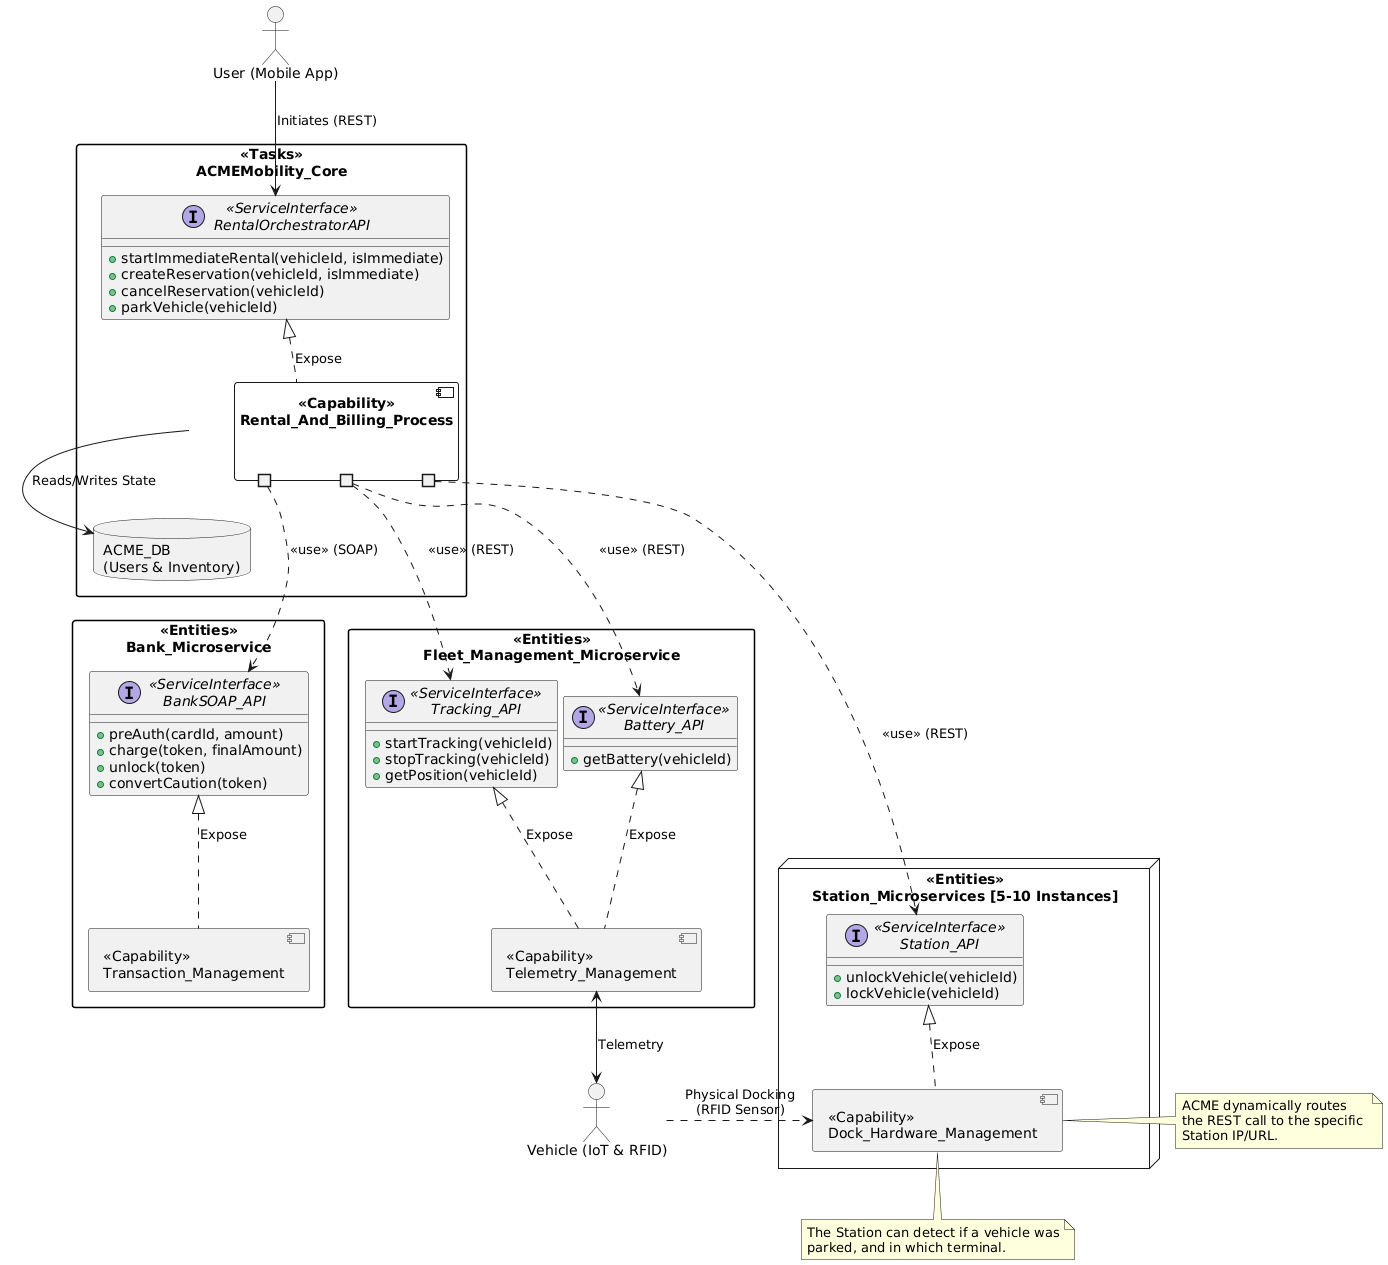
\includegraphics[width=\linewidth,height=1\textheight,keepaspectratio]{../diagrams/diagram-SOA-UML.png}
    \caption{Diagramma SOA in UML.}\label{fig:soa-uml}
\end{figure}

\section{Metodologie e Dati}\label{sec:methods}


\section{Risultati}\label{sec:results}


%\cref{fig:host_performance_img} mostra spesso un picco in casa, ma suggerisce
%anche crescite iniziate prima.
%
%\begin{figure}[H]
%    \centering
%    \includegraphics[width=\linewidth]{../../docs/img/Host_Performance_1996_2024.png}
%    \caption{Performance 1988--2024 per alcuni Pesi host}
%    \label{fig:host_performance_img}
%\end{figure}


\section{Conclusione}
\label{sec:conclusion}


% IEEE bibliography style
\bibliographystyle{IEEEtran}
\bibliography{biblio}

\end{document}
